\documentclass[brazilian, fleqn]{article}

\usepackage{babel}
\usepackage[utf8]{inputenc}
\usepackage[T1]{fontenc}
\usepackage{lmodern}

\usepackage{amssymb,amsfonts,amsmath}

\usepackage{tikz}
\usetikzlibrary{tikzmark}
\usetikzlibrary{calc,intersections}

\DeclareMathOperator{\sen}{sen}

\usepackage[left=2cm, bottom=2cm, right=1.5cm, top=1.5cm]{geometry}

%https://tex.stackexchange.com/a/224014
\setlength{\jot}{1em}

\renewcommand{\vec}[1]{\overrightarrow{#1}}

\allowdisplaybreaks[1]

\begin{document}

No tetraedro \(ABCD\), sejam \(M\), \(N\) e \(P\), respectivamente,
os pontos médios de \(BD\), \(CD\) e \(AC\), e \(G\) o baricentro do triângulo \(MNP\).
\begin{enumerate}
    \item Exprima \(\vec{BG}\) como combinação linear de \(\vec{BA}\), \(\vec{BC}\) e \(\vec{BD}\)
    \item Calcule \(m\) para que o ponto \(X=B+m\vec{BG}\) pertença ao plano da face \(ACD\)
\end{enumerate}

\begin{center}

    \begin{minipage}{0.45\textwidth}
        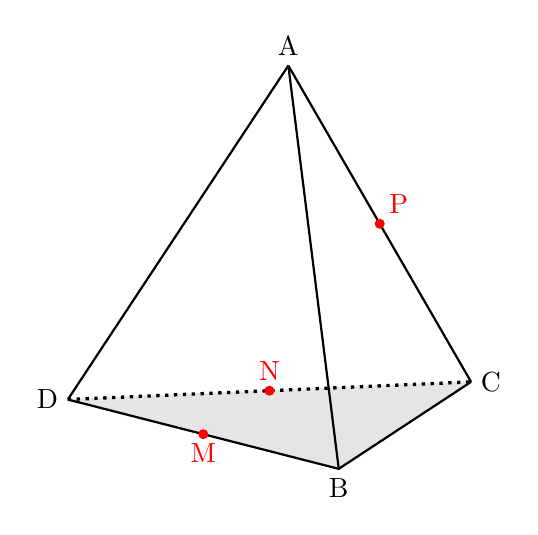
\begin{tikzpicture}[scale=1.6]
            \coordinate (A) at (0.6,0.95);
            \coordinate (B) at (2.75,0.4);
            \coordinate (C) at (3.8,1.09);
            \coordinate (O) at (2.35, 3.6);
            \draw [thick] (O) -- (A);
            \filldraw [gray!20] (A) -- (B) -- (C) -- cycle;
            \draw [thick] (A) -- (B) -- (C);
            \draw [very thick, dotted] (A) -- (C);
            \draw [thick] (O) -- (B);
            \draw [thick] (O) -- (C);
            \node [above]  at (O) {A};
            \node [below]  at (B) {B};
            \node [left]   at (A) {D};
            \node [right]  at (C) {C};
            \filldraw [red] ($(B)!0.5!(A)$) circle (1pt) node [below] {M};
            \filldraw [red] ($(A)!0.5!(C)$) circle (1pt) node [above] {N};
            \filldraw [red] ($(O)!0.5!(C)$) circle (1pt) node [above right] {P};
        \end{tikzpicture}
    \end{minipage}
    %
    \begin{minipage}{0.45\textwidth}
        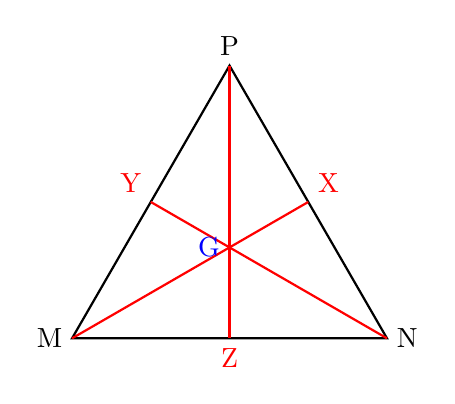
\begin{tikzpicture}[scale=2]
            \coordinate (M) at (0,0);
            \coordinate (N) at (2,0);
            \coordinate (P) at (1,{sqrt(3)});
            \draw[thick] (M) -- (N) -- (P) -- cycle;
            \node [left] at (M) {M};
            \node [right] at (N) {N};
            \node [above] at (P) {P};
            \coordinate (Y) at ($(M) !0.5! (P)$);
            \coordinate (X) at ($(P) !0.5! (N)$);
            \coordinate (Z) at ($(M) !0.5! (N)$);
            \node [red,below] at (Z) {Z};
            \node [red,above right] at (X) {X};
            \node [red,above left] at (Y) {Y};
            \draw [thick, red, name path=MX] (M) -- (X);
            \draw [thick, red] (N) -- (Y);
            \draw [thick, red, name path=PZ] (P) -- (Z);
            \path [name intersections={of=MX and PZ,by=G}];
            \node [blue,left] at (G) {G};
        \end{tikzpicture}
    \end{minipage} \notag \\
    %
\end{center}

\section{Resolução do item 1}

\begin{gather}
    \vec{BG}= \vec{BM}+\vec{MG}=\frac{\vec{BD}}{2}+\vec{MG} \\
    \vec{MG}=\alpha \vec{MN}+\beta \vec{MP} \\
    \begin{aligned}[t]
        \vec{MN}&=\vec{MD}+\vec{DN} =\frac{\vec{BD}}{2}+\frac{\vec{DC}}{2} \\
                &=\frac{\vec{BD}}{2}-\frac{\vec{BD}}{2}+\frac{\vec{BC}}{2} \\
                &=\frac{\vec{BC}}{2}
    \end{aligned} \\
    \begin{aligned}[t]
        \vec{MP}&=\vec{MB}+\vec{BC}+\vec{CP}=-\frac{\vec{BD}}{2}+\vec{BC}+\frac{\vec{CA}}{2} \\
                &=-\frac{\vec{BD}}{2}+\vec{BC}-\frac{\vec{BC}}{2}+\frac{\vec{BA}}{2} \\
                &=\frac{\vec{BA}}{2}+\frac{\vec{BC}}{2}-\frac{\vec{BD}}{2}
    \end{aligned} \\
    \begin{aligned}[t]
        \vec{BG}&=\frac{\vec{BD}}{2}+\alpha \frac{\vec{BC}}{2}+\beta \frac{\vec{BA}}{2}+\beta \frac{\vec{BC}}{2}-\beta \frac{\vec{BD}}{2} \\
                &=\frac{\beta}{2}\vec{BA}+\frac{1}{2}(\alpha+\beta)\vec{BC}+\frac{1}{2}(1-\beta)\vec{BD}
    \end{aligned} \\
    \vec{MG}=\alpha \vec{MN}+\beta \vec{MP} \\
    \vec{MG}=\lambda \vec{MX} \\
    \begin{aligned}[t]
        \vec{MX}&=\vec{MN}+\vec{NX}=\vec{MN}+\frac{NP}{2}\\
                &=\vec{MN}-\frac{\vec{MN}}{2}+\frac{\vec{MP}}{2} \\
                &=\frac{\vec{MN}}{2}+\frac{\vec{MP}}{2}
    \end{aligned} \\
    \vec{MG}=\frac{\lambda}{2}(\vec{MN}+\vec{MP})\\
    \vec{MG}=\vec{MN}+\vec{NG} \\
    \vec{NG}=\sigma \vec{NY} \\
    \vec{NY} =\vec{NM}+\vec{MY} =-\vec{MN}+\frac{\vec{MP}}{2} \\
    \vec{NG}= \sigma\left(-\vec{MN}+\frac{\vec{MP}}{2}\right)\\
    \vec{MG}=\vec{MN}+\sigma\left(-\vec{MN}+\frac{\vec{MP}}{2}\right)\\
    \vec{MG}=(1-\sigma)\vec{MN}+\frac{\sigma}{2}\vec{MP} \\
    \begin{cases}
        1-\sigma &= \frac{\lambda}{2}\\
        \frac{\sigma}{2}&=\frac{\lambda}{2}
    \end{cases} \implies
    \lambda = \sigma = \frac{2}{3}\\
    \alpha = \beta = \frac{1}{3} \\
    \vec{BG}=\frac{\vec{BA}}{6}+\frac{\vec{BC}}{3}+\frac{\vec{BD}}{3}
\end{gather}

\section{Resolução do item 2}
\begin{itemize}
    \item Temos
        \[
            \vec{BG}=\frac{\vec{BA}}{6}+\frac{\vec{BC}}{3}+\frac{\vec{BD}}{3}
        \]
    \item Queremos determinar \(m\) para que o ponto \(X=B+m\vec{BG}\) pertença ao plano da face \(ACD\)
\end{itemize}
\begin{center}
    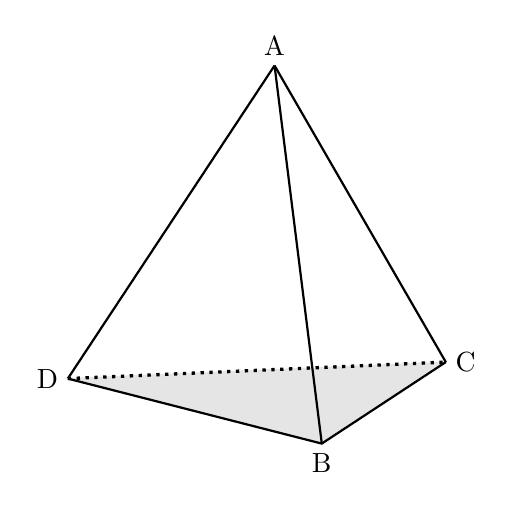
\begin{tikzpicture}[scale=1.5]
        \coordinate (A) at (0.6,0.95);
        \coordinate (B) at (2.75,0.4);
        \coordinate (C) at (3.8,1.09);
        \coordinate (O) at (2.35, 3.6);
        \draw [thick] (O) -- (A);
        \filldraw [gray!20] (A) -- (B) -- (C) -- cycle;
        \draw [thick] (A) -- (B) -- (C);
        \draw [very thick, dotted] (A) -- (C);
        \draw [thick] (O) -- (B);
        \draw [thick] (O) -- (C);
        \node [above]  at (O) {A};
        \node [below]  at (B) {B};
        \node [left]   at (A) {D};
        \node [right]  at (C) {C};
        % \filldraw [red] ($(B)!0.5!(A)$) circle (1pt) node [below] {M};
        % \filldraw [red] ($(A)!0.5!(C)$) circle (1pt) node [above] {N};
        % \filldraw [red] ($(O)!0.5!(C)$) circle (1pt) node [above right] {P};
    \end{tikzpicture}
\end{center}
\begin{gather}
    \vec{BX}=\frac{m}{6}\vec{BA}+\frac{m}{3}\vec{BC}+\frac{m}{3}\vec{BD}\\
    \alpha \vec{DX}+\beta \vec{AC}+\gamma \vec{CD} = \vec{0} \\
    \begin{aligned}[t]
        \vec{DX}&=\vec{DB}+\vec{BX}\\
                &=-\vec{BD}+\vec{BX}\\
                &=-\vec{BD}+\frac{m}{6}\vec{BA}+\frac{m}{3}\vec{BC}+\frac{m}{3}\vec{BD}\\
                &=\frac{m}{6}\vec{BA}+\frac{m}{3}\vec{BC}+\left(\frac{m}{3}-1\right)\vec{BD}
    \end{aligned} \\
    \vec{AC}=\vec{AB}+\vec{BC}=-\vec{BA}+\vec{BC}\\
    \vec{CD}=\vec{CB}+\vec{BD}=-\vec{BC}+\vec{BD}\\
    \alpha \left[\frac{m}{6}\vec{BA}+\frac{m}{3}\vec{BC}+\left(\frac{m}{3}-1\right)\vec{BD}\right]+
    \beta \left(-\vec{BA}+\vec{BC}\right)+ \gamma \left(-\vec{BC}+\vec{BD}\right) = \vec{0} \\
    \left(\alpha\frac{m}{6}-\beta\right)\vec{BA}+\left(\alpha\frac{m}{3}+\beta-\gamma\right)\vec{BC}+
    \left[\alpha\left(\frac{m}{3}-1\right)+\gamma\right]\vec{BD}=\vec{0} \\
    \begin{cases}
        \alpha\frac{m}{6}-\beta &=0 \\
        \alpha\frac{m}{3}+\beta-\gamma &=0 \\
        \alpha\left(\frac{m}{3}-1\right)+\gamma &=0
    \end{cases} \\
    \begin{vmatrix}
        \frac{m}{6} & -1 & 0 \\
        \frac{m}{3} & 1 & -1 \\
        \frac{m}{3}-1 & 0 & 1
    \end{vmatrix} = 0 \\
    \frac{m}{6}+\frac{m}{3}-1+\frac{m}{3}=0 \\
    m=\frac{6}{5}
\end{gather}

\section{Atividade}

No tetraedro \(ABCD\), sejam \(M\), \(N\) e \(P\), respectivamente,
os pontos médios de \(BC\), \(CD\) e \(AC\), e \(G\) o baricentro do triângulo \(MNP\).
\begin{enumerate}
    \item Exprima \(\vec{CG}\) como combinação linear de \(\vec{CA}\), \(\vec{CB}\) e \(\vec{CD}\)
    \item Calcule \(m\) para que o ponto \(X=C+m\vec{CG}\) pertença ao plano da face \(ABD\)
\end{enumerate}

\end{document}
